\begin{strip}
\centering
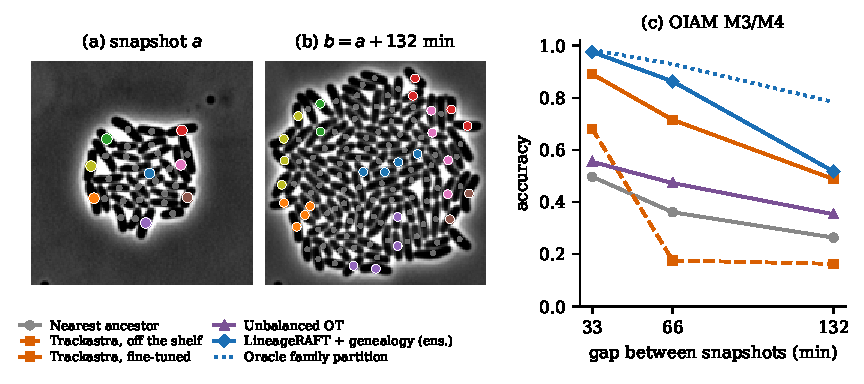
\includegraphics[width=\linewidth]{fig/teaser.pdf}
\captionsetup{hypcap=false}
\captionof{figure}{\textbf{Two-snapshot ancestry.} (a) A \emph{C.~glutamicum} microcolony and (b) the same colony 132 minutes later; eight ancestors in (a) and their descendants in (b) are coloured, all other cells are grey. Descendant families are displaced and interleaved by growth. (c) Accuracy on One-in-a-Million (OIAM) movies M3/M4 (rows of \cref{tab:oiam}; \ours: three-seed ensemble with genealogy decoder). A recent learned tracker given ground-truth masks falls below nearest assignment from 66 minutes on unless fine-tuned at each gap on annotated lineage; unbalanced optimal transport gains little. Family registration with single-snapshot genealogy stays above all of them and approaches an oracle that knows the family partition at short gaps.}
\captionsetup{hypcap=true}
\label{fig:teaser}
\end{strip}
